\documentclass[11pt]{article}
\usepackage[margin=1in]{geometry}
\usepackage{booktabs}
\usepackage{graphicx}
\usepackage{amsmath}
\usepackage{hyperref}
\graphicspath{{figures/}}
\title{Hazard--Placement Ablation on a Sparse Chain of Communities}
\author{}
\date{11 July 2026}

\begin{document}
\maketitle

\section{Research question}
This experiment asks whether the early-arrival bias of the MicroMacro approximation is caused primarily by replacing the active-edge transmission hazard with a prevalence-based aggregate hazard, by placing imports uniformly inside a destination community, or by an interaction between these mechanisms. It is a causal ablation on one fixed baseline family, not a general robustness study.

\section{Experimental design}
Each of 100 paired replications used a newly generated chain of $L=10$ connected random communities with $n=100$ nodes, internal mean degree approximately $6$, and $k=5$ inter-community edges per adjacent pair. Parameters were $\beta_{\rm in}=\beta_{\rm out}=0.003$, $\gamma=0$, $\tau_{\rm micro}=1$, and $T_{\rm end}=4000$. All five modes within a replication shared the network, inter-community edges, initial node, and initial state. Deterministic, variant-specific random-number streams were used for events, macro budgets, pair selection, and placement. Pairing therefore controls network and initialization variability but is not event-by-event common-random-number coupling.

The five modes were Full Micro; exact active-edge hazard with exact edge-conditioned placement; exact hazard with uniform susceptible placement; aggregate prevalence hazard with static edge-weighted susceptible boundary placement; and aggregate hazard with uniform susceptible placement. Full Micro and the production MicroMacro implementation were not modified. The isolated ablation scheduler uses exact competition between microscopic and macro exponential clocks; consequently its aggregate/uniform mode reproduces the production hazard and placement semantics, but deliberately excludes midpoint synchronization error.

\section{Mathematical definitions}
For directed community pair $i\to j$, the oracle hazard is
\[
a^*_{ij}(x)=\beta_{\rm out}\sum_{(u,v)\in E_{ij}}w_{uv}
\mathbf{1}\{X_u=I,X_v=S\},
\]
and exact placement assigns a susceptible endpoint $v$ probability proportional to its incoming weight from currently infected source endpoints. The aggregate hazard is
\[
\lambda_{ij}(t)=\beta_{\rm macro}W_{ij}\bar i_i(t)\bar s_j(t).
\]
Boundary-aware placement is proportional to static incoming inter-community weight among susceptible destination boundary nodes. It is not exact placement.

The nominal factorial cell ``aggregate hazard plus exact placement'' is not generally defined: $\lambda_{ij}>0$ can hold while $a^*_{ij}=0$, in which case no active microscopic edge and no exact edge-conditioned target distribution exist. This cell was therefore omitted rather than supplied with a silent uniform fallback.

\section{Sanity checks}
All eight automated tests passed. They verify exact hazards against brute-force explicit-edge sums (including 25 random states), exact-placement support and normalization, boundary-placement weights and support, zero exact hazard without active edges, absence of the invalid aggregate/exact configuration, and deterministic reproduction. No null event or silent fallback occurred in the final experiment.

The oracle control passed its statistical gate. Its completion probability equalled Full Micro (both $1.00$), relative Wasserstein distance for $T_{\rm last}$ was $0.0138$, and paired $\Delta$RMST was $7.5$ time units with 95\% bootstrap CI $[-93.6,120.3]$. Thus no detectable scheduler discrepancy remains at the resolution of 100 replications.

\section{Results}
All modes completed all 100 replications before $T_{\rm end}$, so completed-only and censoring-aware terminal-time summaries coincide here. Nevertheless, RMST is retained as the primary contrast because it remains valid if later settings introduce censoring.

\begin{table}[ht]
\centering
\small
\begin{tabular}{lrrrr}
\toprule
Mode & Mean $T_{\rm last}$ & W1 & Relative W1 & $\Delta$RMST \\
\midrule
Full Micro & 2936.7 & 0.0 & 0.000 & 0.0 \\
Exact/exact & 2944.3 & 40.4 & 0.014 & 7.5 \\
Exact/uniform & 2775.5 & 163.6 & 0.056 & -161.2 \\
Aggregate/boundary & 2735.5 & 203.5 & 0.069 & -201.2 \\
Aggregate/uniform & 2715.9 & 220.8 & 0.075 & -220.8 \\
\bottomrule
\end{tabular}
\caption{Terminal-arrival summaries. W1 is measured against Full Micro.}
\end{table}

\begin{figure}[ht]
\centering
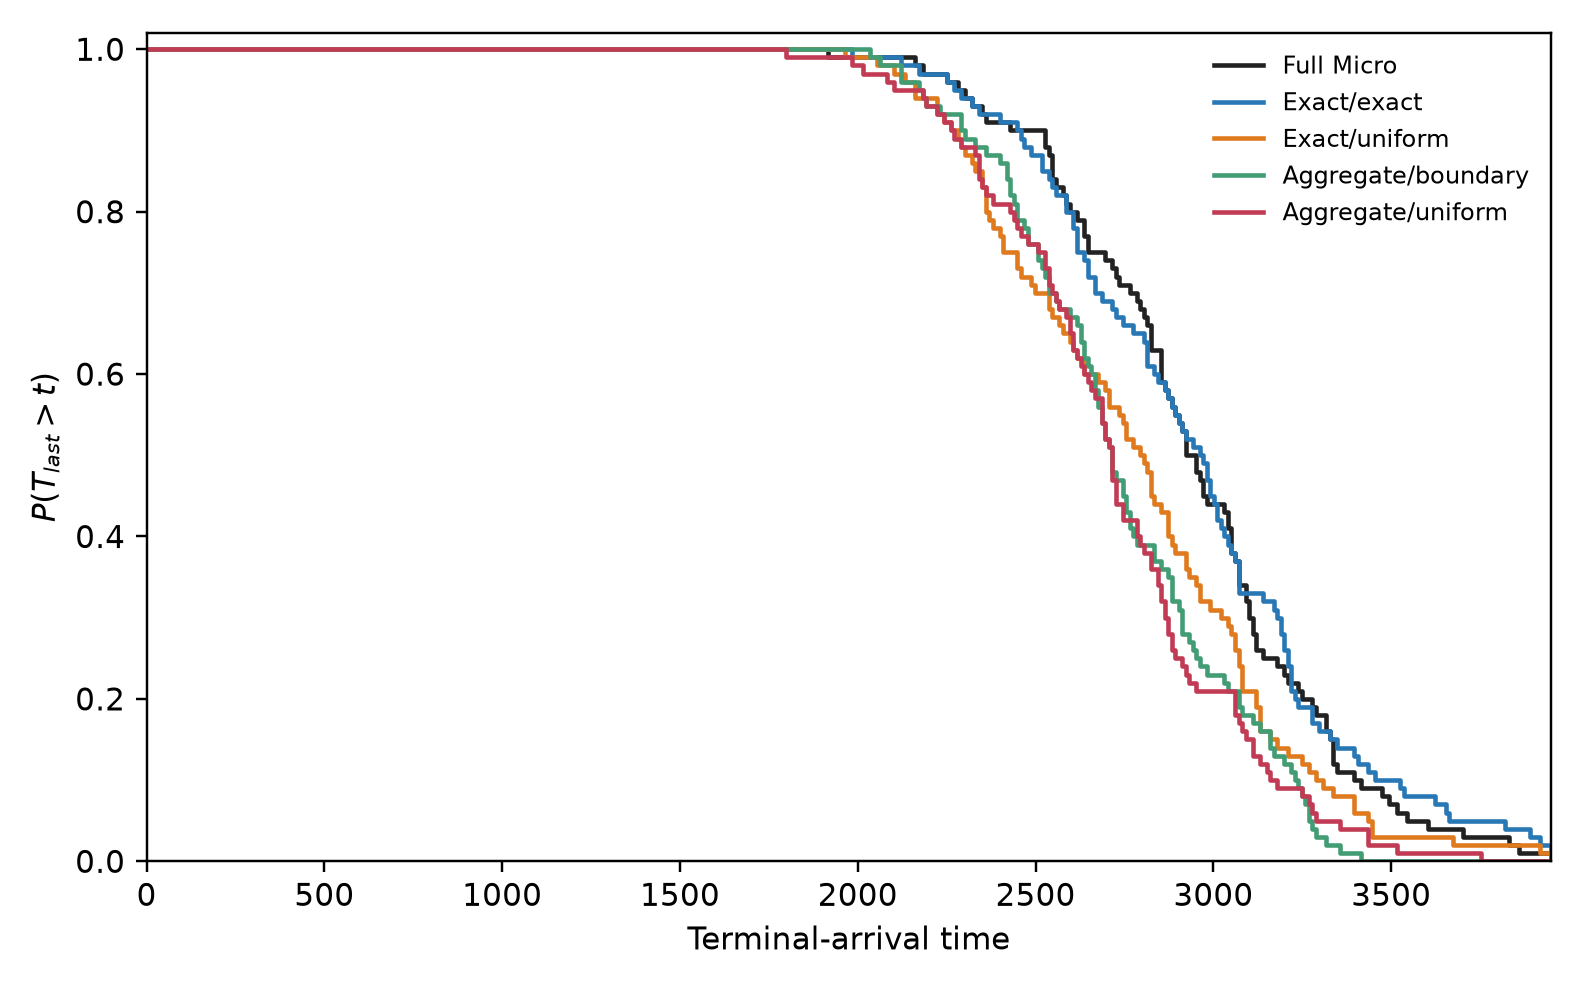
\includegraphics[width=.49\textwidth]{survival.png}
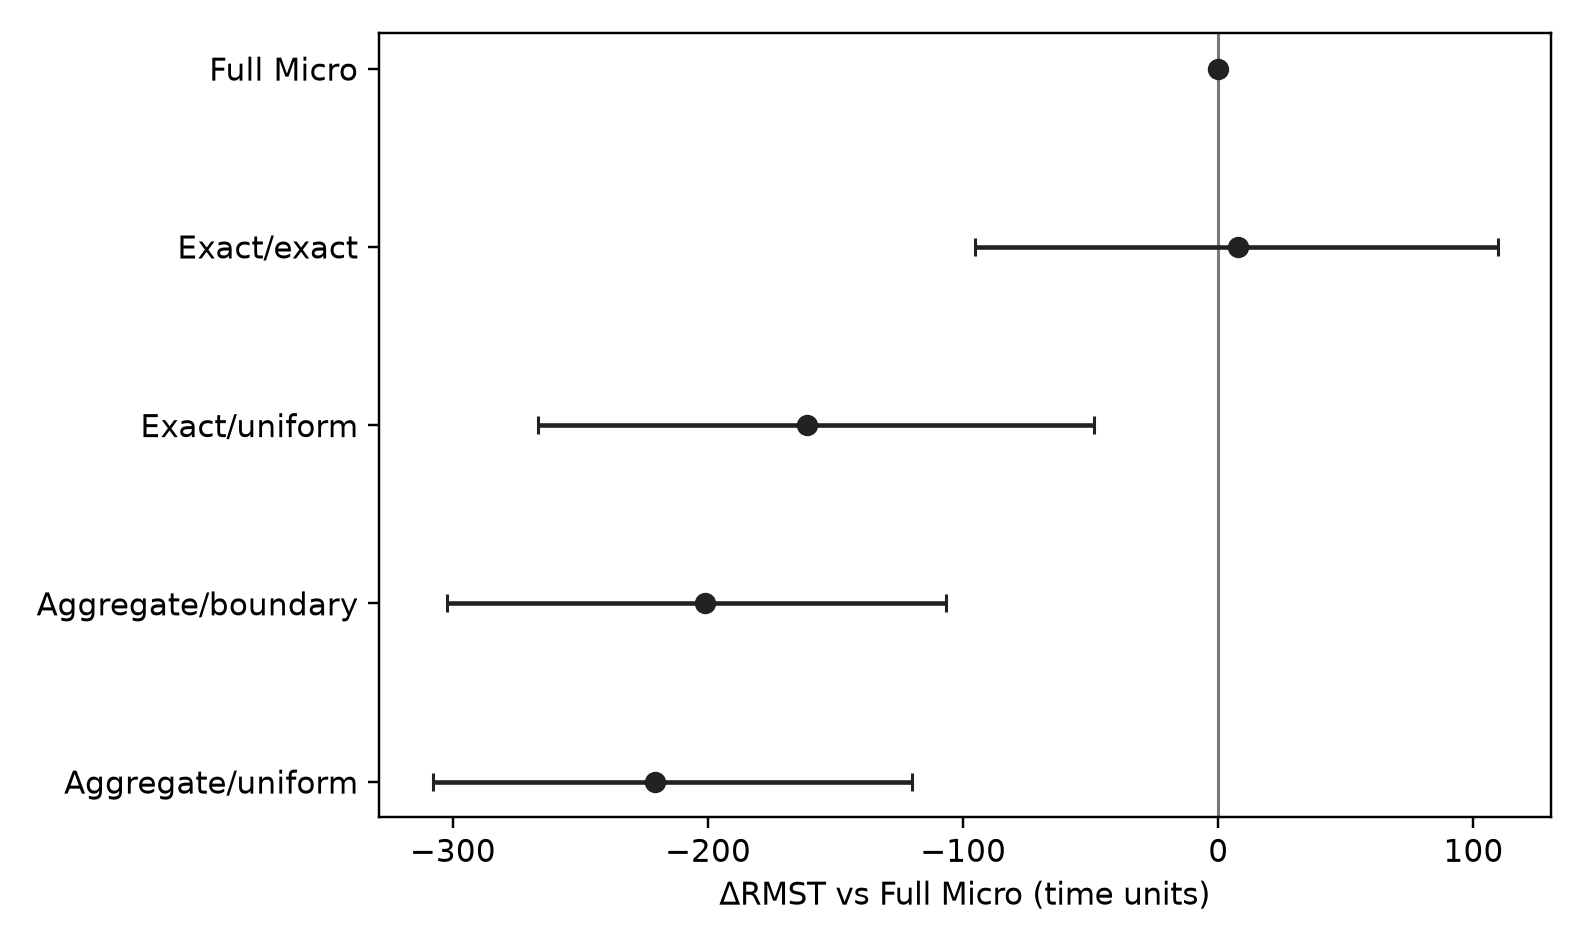
\includegraphics[width=.49\textwidth]{rmst_shift.png}
\caption{Terminal-arrival survival curves (left) and paired RMST shifts with 95\% bootstrap intervals (right).}
\end{figure}

\begin{figure}[ht]
\centering
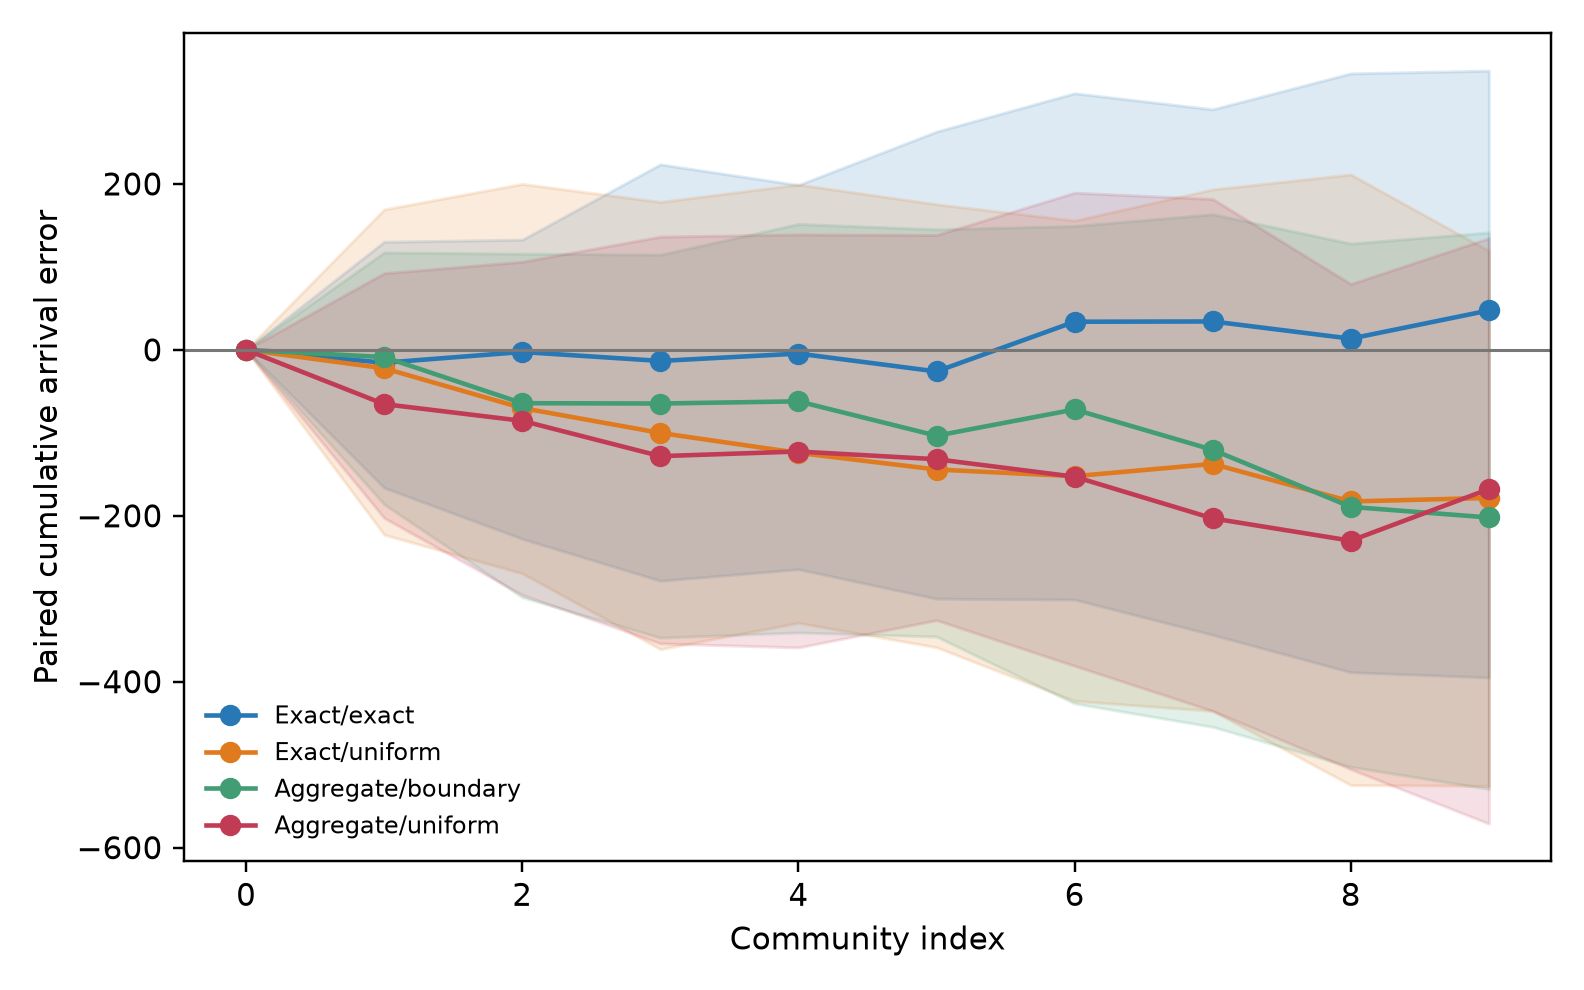
\includegraphics[width=.49\textwidth]{cumulative_error.png}
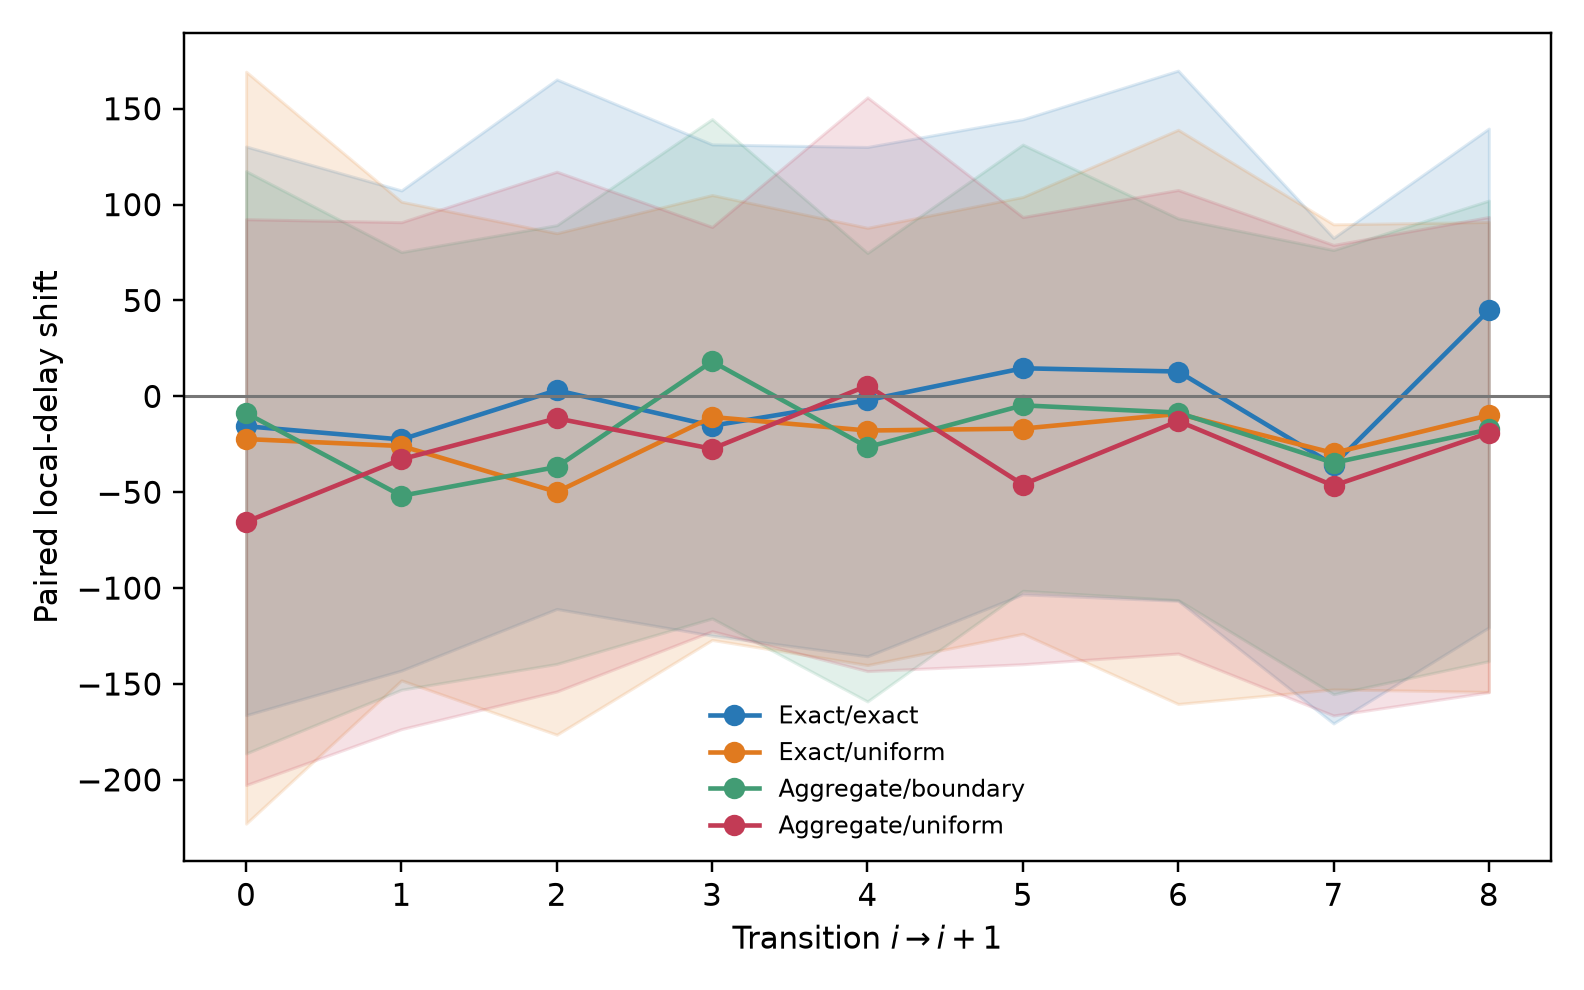
\includegraphics[width=.49\textwidth]{local_delay_shift.png}
\caption{Layer-wise cumulative arrival error (left) and local-delay shifts (right). Lines are paired medians and bands are paired interquartile ranges across 100 replications.}
\end{figure}

\section{Placement effect}
With exact event hazards fixed, replacing exact endpoint placement by uniform susceptible placement changed RMST by $-168.8$ time units (95\% CI $[-274.5,-56.1]$). The effect accumulates along the chain rather than appearing only at the terminal community. Uniform placement can seed an interior node that is better positioned for subsequent within-community spreading or for reaching the next boundary than the endpoint selected by an actual active edge. Import placement is therefore a statistically supported contributor to early arrival in this baseline.

\section{Hazard effect}
The boundary-aware aggregate mode differed from exact/exact by $-208.8$ time units (95\% CI $[-310.0,-112.2]$). This contrast reduces placement mismatch but is not a pure factorial hazard effect, because boundary placement uses static incoming weights rather than the dynamic infected-edge-conditioned distribution. It nevertheless demonstrates that prevalence aggregation plus its necessarily approximate boundary placement produces substantial early-arrival bias even when imports are restricted to plausible gateway nodes.

Aggregate/boundary and aggregate/uniform generated 63,298 and 295,719 synchronization intervals, respectively, with $\lambda_{ij}>0$ and $a^*_{ij}=0$. They also generated 245 and 561 actual imports in states where exact placement would have been undefined. These cases were logged explicitly; the boundary mode gated directions with no susceptible boundary target to zero.

\begin{figure}[ht]
\centering
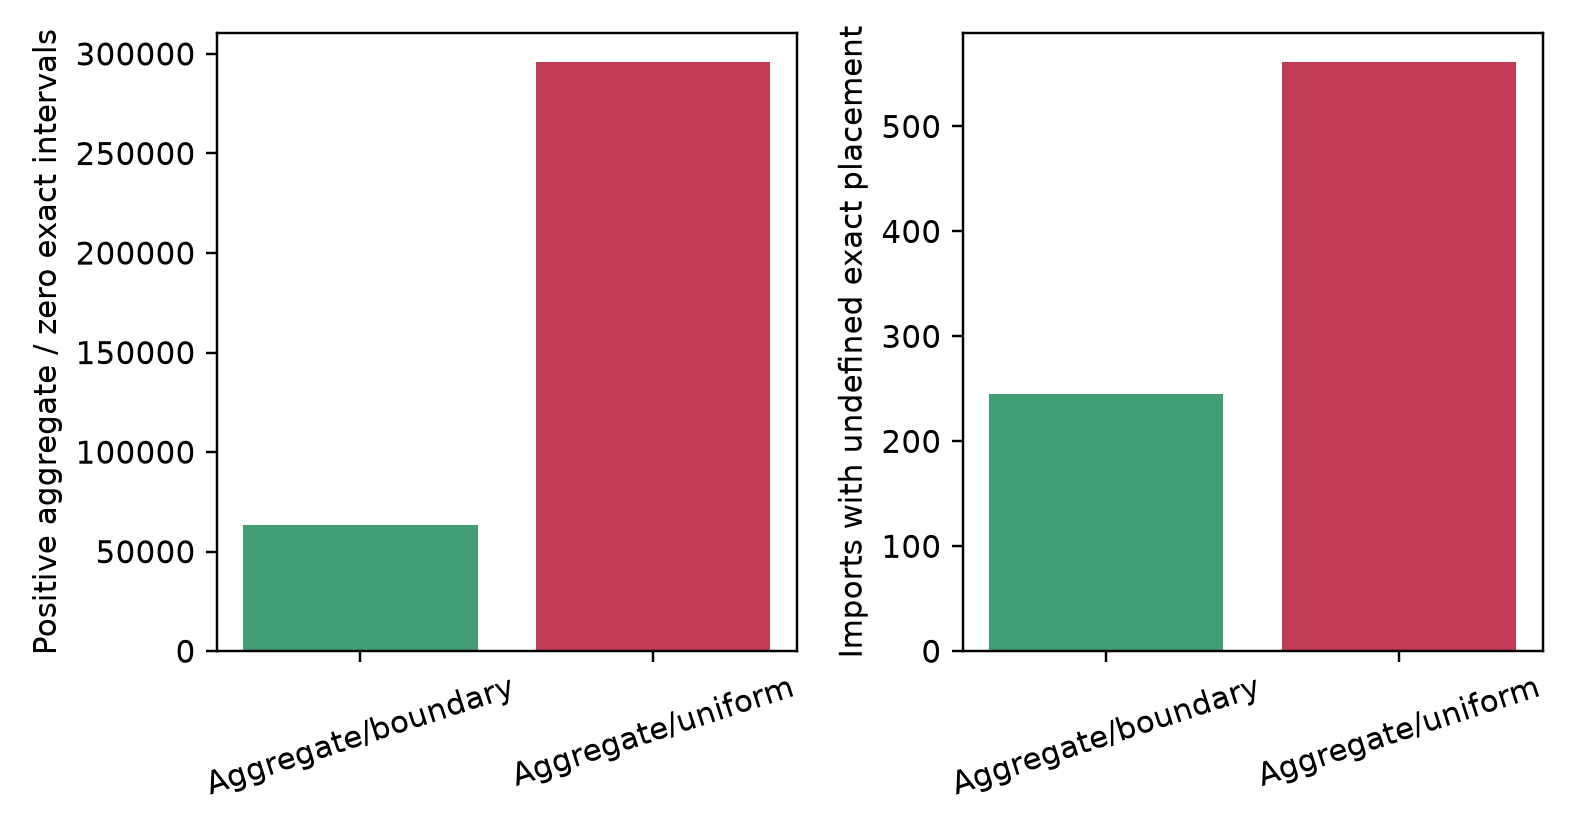
\includegraphics[width=.49\textwidth]{premature_hazard.png}
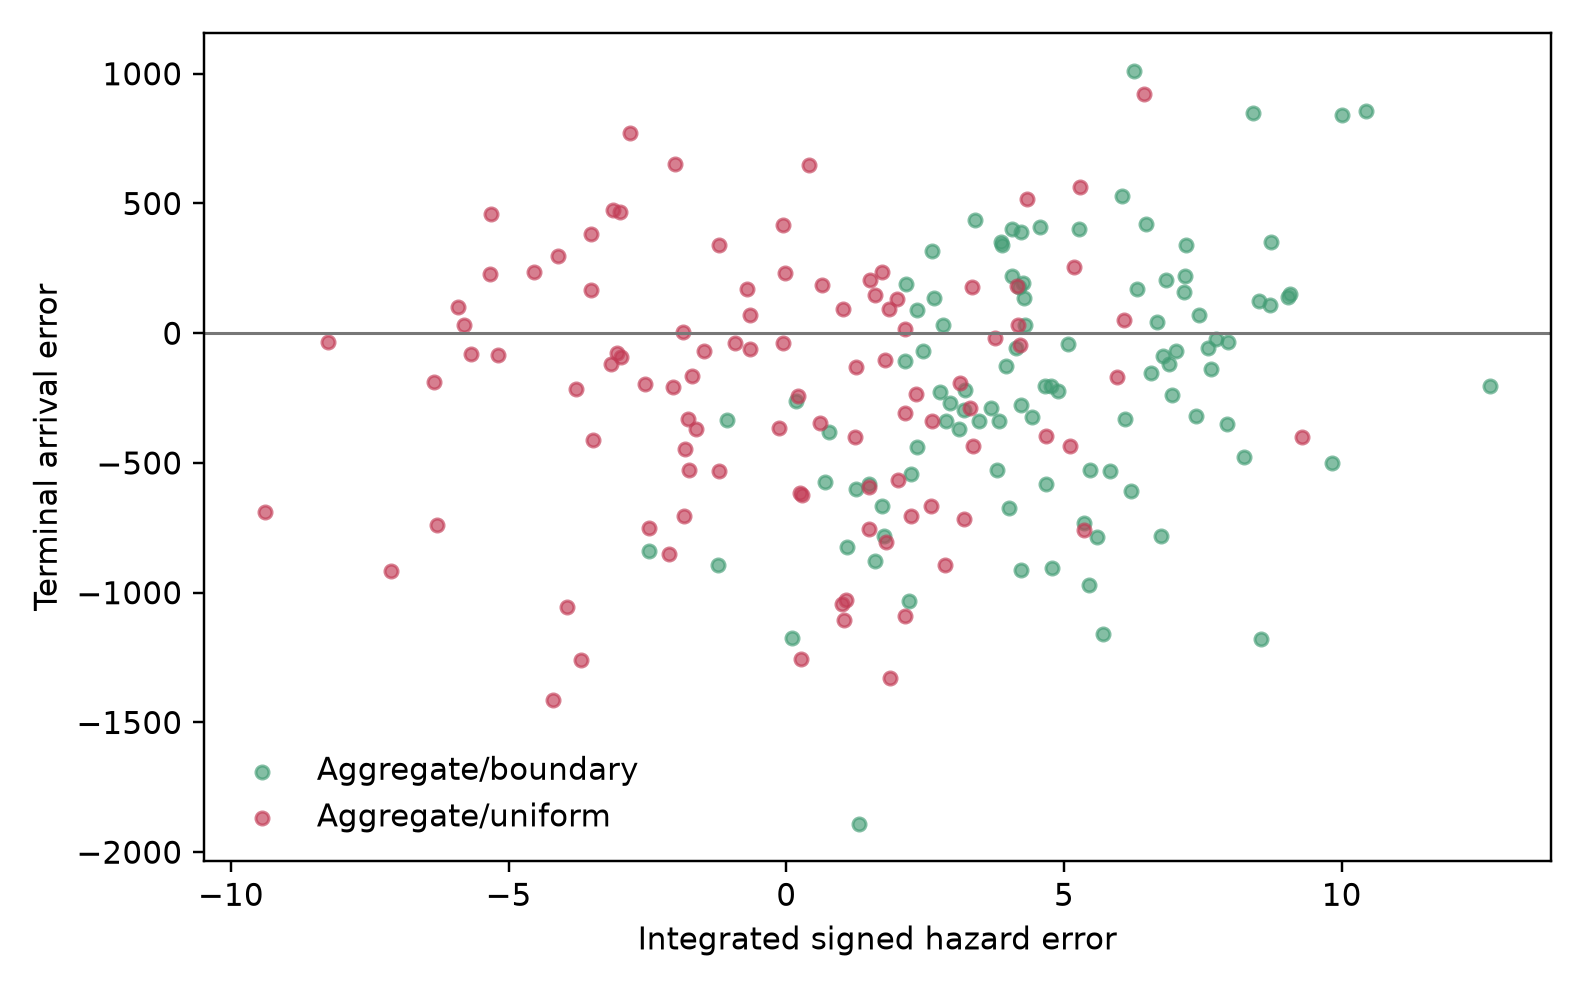
\includegraphics[width=.49\textwidth]{hazard_vs_arrival.png}
\caption{Premature-hazard diagnostics (left) and per-replication integrated signed hazard error versus terminal-arrival error (right). Counts depend on each mode's endogenous path and must not be interpreted as paired observations of one common state trajectory.}
\end{figure}

\section{Interaction}
The full aggregate/uniform error was $-220.8$ time units (95\% CI $[-315.5,-126.8]$). Once aggregate hazard and boundary placement were already used, changing boundary placement to uniform changed RMST by only $-19.6$ (95\% CI $[-114.2,77.2]$). This is much smaller than the $-168.8$ exact-hazard placement effect. The difference between these placement contrasts was $149.2$ (95\% CI $[5.7,290.1]$). Hence the two errors are not additive: they interact, overlap, or saturate along the propagation path. It would be incorrect to attribute the full $-220.8$ shift by summing the two marginal contrasts.

\begin{figure}[ht]
\centering
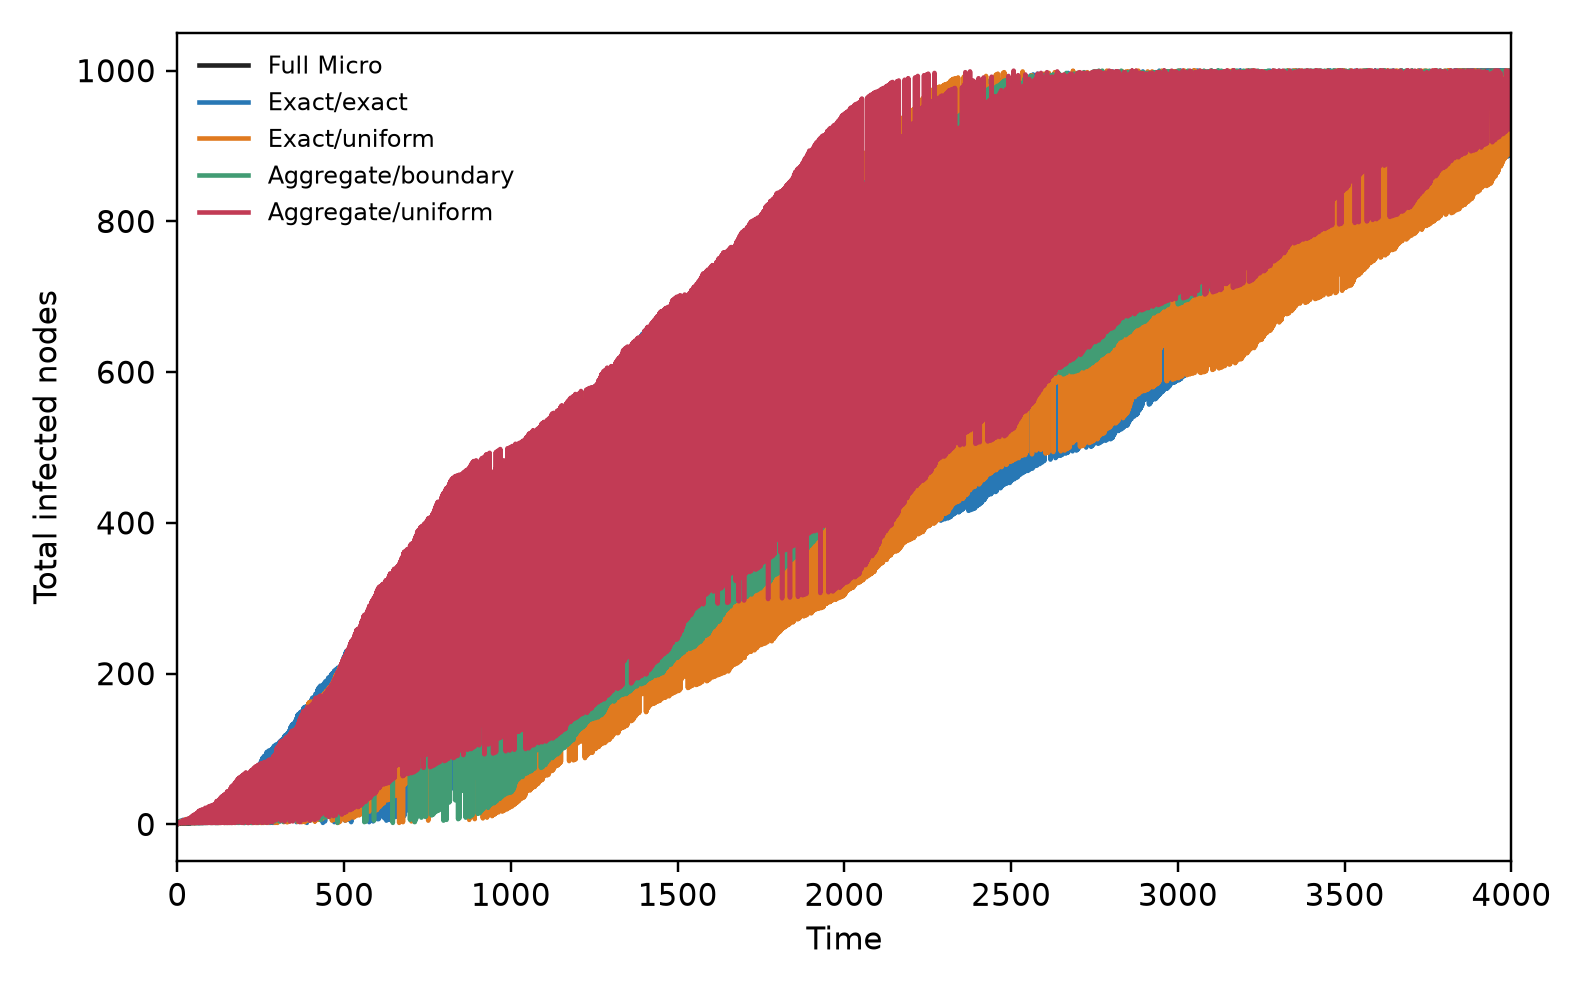
\includegraphics[width=.72\textwidth]{infected_dynamics.png}
\caption{Pointwise median total infected count with interquartile bands. Because $\gamma=0$, infected counts are cumulative and monotone. The plot describes process dynamics; distributional claims rely on the paired arrival-time metrics above.}
\end{figure}

\section{Limitations}
The exact aggregate-hazard/exact-placement factorial cell is mathematically undefined in some states, so the hazard contribution cannot be identified independently of every placement approximation. The boundary contrast is the closest well-defined proxy, not an exact decomposition. Hazard diagnostics are accumulated on each mode's own endogenous trajectory, and their raw counts are therefore descriptive rather than controlled state-by-state comparisons. This experiment covers one sparse-chain baseline with no recovery. It does not establish behavior across interface width, community size, recovery rate, or synchronization interval. Runtime values were logged for reproducibility but are not used for speedup claims because the experimental scheduler prioritizes diagnosis rather than optimization.

\section{Recommended next experiment}
The next useful experiment is a state-replay hazard audit: save microscopic states from Full Micro at fixed observation times and evaluate both $a^*_{ij}$ and $\lambda_{ij}$ on those same states without allowing either approximation to alter the trajectory. This would estimate pure instantaneous rate abstraction error under a common state distribution. A subsequent gateway-distance experiment could then test the proposed mechanism behind the placement effect by stratifying import endpoints by distance to the next interface.

\section{Conclusion}
The oracle architecture is statistically consistent with Full Micro. Uniform import placement alone produces a clear early-arrival bias under exact hazards. Aggregate prevalence hazard with boundary-aware placement produces a similarly clear, somewhat larger point estimate, but its confidence interval overlaps the placement-effect interval and the contrast is not a pure factorial hazard effect. The current aggregate/uniform error is substantial (relative W1 $7.5\%$), yet it is not the sum of two independent errors. The defensible conclusion is that both mechanisms matter in this sparse chain and interact strongly; this experiment does not support assigning a unique percentage of the total bias to either component.

\end{document}
